\documentclass{article}
\usepackage{tikz}
\usetikzlibrary{shapes.geometric, arrows}

\begin{document}
\begin{figure}[h]
\centering
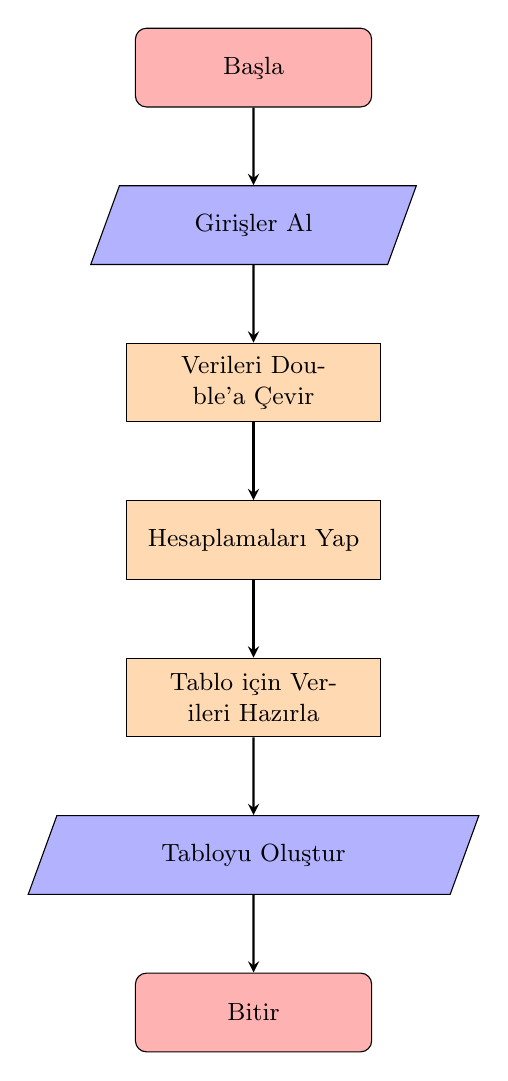
\begin{tikzpicture}[node distance=2cm, every node/.style={font=\small}]

% Define styles for the flowchart
\tikzstyle{startstop} = [rectangle, rounded corners, minimum width=3cm, minimum height=1cm, text centered, draw=black, fill=red!30]
\tikzstyle{io} = [trapezium, trapezium left angle=70, trapezium right angle=110, minimum width=3cm, minimum height=1cm, text centered, draw=black, fill=blue!30]
\tikzstyle{process} = [rectangle, minimum width=3cm, minimum height=1cm, text centered, text width=3cm, draw=black, fill=orange!30]
\tikzstyle{arrow} = [thick,->,>=stealth]

% Nodes
\node (start) [startstop] {Başla};
\node (input) [io, below of=start] {Girişler Al};
\node (convert) [process, below of=input] {Verileri Double'a Çevir};
\node (calc) [process, below of=convert] {Hesaplamaları Yap};
\node (prepare) [process, below of=calc] {Tablo için Verileri Hazırla};
\node (table) [io, below of=prepare] {Tabloyu Oluştur};
\node (end) [startstop, below of=table] {Bitir};

% Arrows
\draw [arrow] (start) -- (input);
\draw [arrow] (input) -- (convert);
\draw [arrow] (convert) -- (calc);
\draw [arrow] (calc) -- (prepare);
\draw [arrow] (prepare) -- (table);
\draw [arrow] (table) -- (end);

\end{tikzpicture}
\caption{Akış Diyagramı}
label{fig:flowchart}
\end{figure}
\end{document}
